%% FEUP THESIS STYLE for LaTeX2e
%% how to use feupteses (English version)
%%
%% FEUP, JCL & JCF, 31 July 2012
%%
%% PLEASE send improvements to jlopes at fe.up.pt and to jcf at fe.up.pt
%%

%%========================================
%% Commands: pdflatex tese
%%           bibtex tese
%%           makeindex tese (only if creating an index)
%%           pdflatex tese
%% Alternative:
%%          latexmk -pdf tese.tex
%%========================================

\documentclass[11pt,a4paper,twoside,openright]{report}

%% For iso-8859-1 (latin1), comment next line and uncomment the second line
\usepackage[utf8]{inputenc}
%\usepackage[latin1]{inputenc}

\usepackage{xcolor}
\usepackage{ifthen}
\usepackage{mathtools}
\usepackage{float}
\usepackage{listings}
\usepackage[]{algorithm2e}
\restylefloat{table}


%% English version

%% MIEIC options
%\usepackage[mieic]{feupteses}
%\usepackage[mieic,juri]{feupteses}
\usepackage[mieic,final]{feupteses}
%\usepackage[mieic,final,onpaper]{feupteses}

%% Additional options for feupteses.sty:
%% - onpaper: links are not shown (for paper versions)
%% - backrefs: include back references from bibliography to citation place

%% Uncomment the next lines if side by side graphics used
%\usepackage[lofdepth,lotdepth]{subfig}
%\usepackage{graphicx}
%\usepackage{float}

%% Include color package
\usepackage{color}
\definecolor{cloudwhite}{cmyk}{0,0,0,0.025}

%% Include source-code listings package
\usepackage{listings}
\lstset{ %
 language=C,                        % choose the language of the code
 basicstyle=\footnotesize\ttfamily,
 keywordstyle=\bfseries,
 numbers=left,                      % where to put the line-numbers
 numberstyle=\scriptsize\texttt,    % the size of the fonts that are used for the line-numbers
 stepnumber=1,                      % the step between two line-numbers. If it's 1 each line will be numbered
 numbersep=8pt,                     % how far the line-numbers are from the code
 frame=tb,
 float=htb,
 aboveskip=8mm,
 belowskip=4mm,
 backgroundcolor=\color{cloudwhite},
 showspaces=false,                  % show spaces adding particular underscores
 showstringspaces=false,            % underline spaces within strings
 showtabs=false,                    % show tabs within strings adding particular underscores
 tabsize=2,	                    % sets default tabsize to 2 spaces
 captionpos=b,                      % sets the caption-position to bottom
 breaklines=true,                   % sets automatic line breaking
 breakatwhitespace=false,           % sets if automatic breaks should only happen at whitespace
 escapeinside={\%*}{*)},            % if you want to add a comment within your code
 morekeywords={*,var,template,new}  % if you want to add more keywords to the set
}

%% Uncomment to create an index (at the end of the document)
%\makeindex

%% Path to the figures directory
%% TIP: use folder ``figures'' to keep all your figures
\graphicspath{{figures/}}

%%----------------------------------------
%% TIP: if you want to define more macros, use an external file to keep them
%some macro definitions

\newboolean{showcomments}
\setboolean{showcomments}{true}
%
\ifthenelse{\boolean{showcomments}}{
    \newcommand{\nb}[2]{
        {\color{red}\small\fbox{\bfseries\sffamily\scriptsize#1}}
        {\color{red}\sffamily\small$\triangleright~$\textit{\small #2}$~\triangleleft$}
    }
}
{\newcommand{\nb}[2]{}}
%
%commands to add comments in the text
\newcommand\af[1]{\nb{Andr\'e}{#1}} % André
\newcommand\ap[1]{\nb{Alexandre}{#1}} % Alex
\newcommand\ra[1]{\nb{Rui}{#1}} % Rui

% format
\newcommand{\class}[1]{{\normalfont\slshape #1\/}}

% entities
\newcommand{\Feup}{Faculdade de Engenharia da Universidade do Porto}

\newcommand{\svg}{\class{SVG}}
\newcommand{\scada}{\class{SCADA}}
\newcommand{\scadadms}{\class{SCADA/DMS}}

%%----------------------------------------

%%========================================
%% Start of document
%%========================================
\begin{document}

%%----------------------------------------
%% Information about the work
%%----------------------------------------
\title{Software Repository Mining Analytics to Estimate Software Component Reliability}
\author{André Freitas - freitas.andre@fe.up.pt}


%% Uncomment next line for date of submission
%\thesisdate{July 31, 2008}

%%Uncomment next line for copyright text if used
%\copyrightnotice{Name of the Author, 2008}

\supervisor{Supervisor}{Rui Maranhão - rma@fe.up.pt}
\supervisor{Co-Supervisor}{Alexandre Perez - alexandre.perez@fe.up.pt}

%% Uncomment next line if necessary
%\supervisor{Second Supervisor}{Name of the Supervisor}

%% Uncomment committee stuff in the final version if used
\committeetext{Approved in oral examination by the committee:}
\committeemember{Chair}{Doctor Hugo José Sereno Lopes Ferreira}
\committeemember{External Examiner}{Doctor Jâcome Miguel Costa da Cunha}
\committeemember{Supervisor}{Doctor Rui Filipe Maranhão de Abreu}
\signature

%% Specify cover logo (in folder ``figures'')
\logo{uporto-feup.pdf}

%% Uncomment next line for additional text  below the author's name (front page)
%\additionalfronttext{Preparação da Dissertação}

%%----------------------------------------
%% Preliminary materials
%%----------------------------------------

% remove unnecssary \include{} commands
\begin{Prolog}
  \chapter*{Abstract}
Finding and fixing software bugs is expensive and has a significant impact in Software development effort. Repositories have hidden predictive information about Software history that can be explored using analytics and machine learning techniques. A Software component can be a file, class or method in terms of granularity. Current research in Mining Software Repositories (MSR) is capable of ranking and listing faulty components at the file granularity. Crowbar is an automatic Software debugging tool that uses a technique named Barinel. Our goals are predicting Software defects with method granularity and improve Crowbar, by mining repositories. 

We have implemented a tool named Schwa, available for free on Github, that is capable of analyzing Git repositories. We are analyzing metrics such as revisions, fixes, authors and the time of commits to feed the prediction model. The analysis of time provides a method to ignore old components. Experimental results shown that for every Software repository, the predictive power of each metric is different. For example, in some projects revisions is more correlated with future defects and in others is fixes. The usage of defect predictions from Schwa in Crowbar reduced the amount of time necessary to rank faulty components. In the Joda Time project the time was reduced from one hour to less than a minute.

This thesis does the following contributions: a method to parse and represent diffs from patches with method granularity for Java; a model to compute defect probabilities; a framework for mining Software repositories; a technique to learn the importance of tracked metrics; a method to evaluate the gain of using defect probabilities in fault localization. 

\chapter*{Resumo}
Encontrar e corrigir bugs tem um grande custo e impacto no esforço em desenvolver Software. Os repositórios escondem informação preditiva sobre o histórico de Software que pode ser explorada recorrendo a técnicas de análise e de machine learning. Um componente de Software pode ser um ficheiro, classe ou método em termos de granularidade. A investigação atual de Mining Software Repositories (MSR) é capaz de classificar e listar componentes defeituosos com a granularidade ao nível do ficheiro. O Crowbar é uma ferramenta que faz depuração automática de Software e usa a técnica Barinel. Os nossos objetivos são prever defeitos em Software com granularidade até ao método e melhorar o Crowbar, ao extrair informação de repositórios.

Foi implementada uma ferramenta denominada de Schwa, disponível livremente no Github, que é capaz de analisar repositórios Git. Estamos a analisar métricas como as revisões, correções de bug, autores e o tempo dos commits para alimentar o modelo de previsão. A análise do tempo permite ignorar componentes mais antigos. Os resultados experimentais demonstraram  que para cada repositório de Software, o poder preditivo de cada métrica é diferente. Por exemplo, em alguns projetos o número de revisões está mais correlacionado com futuros defeitos e em outros é o número de correções de bugs. A utilização das previsões de defeito do Schwa no Crowbar reduziu o tempo necessário para classificar componentes faltosos. No projecto Joda Time o tempo foi reduzido de uma hora para menos de um minuto.

Esta tese faz as seguintes contribuições: um método para interpretar e representar diffs de patches com a granularidade ao método; um modelo para calcular probabilidades de defeito; uma framework para minar repositórios de Software; uma técnica para aprender a importância das métricas analisadas; um método para avaliar o ganho de usar as probabilidade de defeito em localização de falhas. % the abstract
  \chapter*{Acknowledgements}

First, I would like to thank my supervisor and co-supervisor, Rui Maranhão and Alexandre Perez for their extraordinary help and mentoring in my dissertation, specially for supporting me on the most difficult challenges. Thanks for accepting me as a dissertation student and for your patience through the last months. I would like to thank my supervisor for the financial aid I received through FCT funding, since it was an important help for me. I would like to thank Nuno Cardoso for helping me through the internals of Crowbar.

Regarding my experiments, I would like to thank the contributions from Shiftforward, Luís Fonseca, Diogo Pinela and Stronsgtep. Thanks Open Source community for making available software for free, that students and researchers frequently use on their projects. Thanks FEUP for having a good environment, teachers and for everyone that indirectly contributed to the success of this thesis that I could not list here.


Finally and not least important, I would like to thank my parents, my family and my girlfriend for always supporting me. They surely gave me an environment to be a better person and pursuing my goals.


\vspace{10mm}
\flushleft{André Freitas}
  % the acknowledgments
  \cleardoublepage
\thispagestyle{plain}

\vspace*{8cm}

\begin{flushright}
   \textsl{``Imagination is more important than knowledge. For knowledge\\ is limited to all we now know and understand, while imagination embraces\\ the entire world, and all there ever will be to know and understand.''} \\
\vspace*{1.5cm}
           Albert Einstein
\end{flushright}
       % initial quotation if desired
  \cleardoublepage
  \pdfbookmark[0]{Table of Contents}{contents}
  \tableofcontents
  \cleardoublepage
  \pdfbookmark[0]{List of Figures}{figures}
  \listoffigures
  \cleardoublepage
  \pdfbookmark[0]{List of Tables}{tables}
  \listoftables
  \chapter*{Abbreviations}
\chaptermark{ABBREVIATIONS}

\begin{flushleft}
\begin{tabular}{l p{0.8\linewidth}}
MSR & Mining Software Repositories\\
TWR & Time-Weighted Risk\\
SCM & Source Control Management \\
SFL & Spectrum-based Fault Localization \\
MDB & Model Based Diagnostic \\
ISTQB & International Software Testing Qualifications Board \\
SaaS & Software as a Service \\
LRU & Least Recented Used \\
URL & Uniform Resource Locator \\
PHP & PHP: Hypertext Preprocessor \\
CSS & Cascading Style Sheets \\
HTML & HyperText Markup Language \\
MIT & Massachusetts Institute of Technology
\end{tabular}
\end{flushleft}

  % the list of abbreviations used
\end{Prolog}

%%----------------------------------------
%% Body
%%----------------------------------------
\StartBody

%% TIP: use a separate file for each chapter
\chapter{Introduction} \label{chap:intro}

\section*{}
We review the state of the art in Mining Software Repositories (MSR),
existing tools and propose a new method to predict defects based on data
extracted from repositories. Also we use this information from defect
prediction to improve the diagnostic accuracy from Crowbar, namely,
the Barinel algorithm.

\section{Context} \label{sec:context}
Software plays an important role for society and in our daily routine, since
we use applications to communicate, manage information, etc. We expect that
these applications behave correctly and we are easily frustrated when they
are defective. Development of software is not a simple task since developers
need to maintain complex code, test and manage expectations of stakeholders
by correctly interpreting requirements. It is estimated that fixing bugs
represent 90\% of development costs \cite{Servant1}.

There are tools that can help developers delivering high quality software,
by automatically reviewing code and analyzing their behaviour. Some of
these tools are Codacy\footnote{\url{https://codacy.com/}},
Crowbar\footnote{\url{http://crowbar.io/}} and
Codeclimate\footnote{\url{https://codeclimate.com/}}. The usage of revision
control systems such as Git, SVN and Mercurial, helps developers tracking
changes on Software and understanding the evolution of components. Tools are
important to developers since they automate and avoid repetitive tasks in
Software development.

With the growing usage of revision control systems, research in MSR evolved
in the last decade and involves the analysis of systems used to support
the development of software such as repositories, issue trackers and
mailing lists \cite{Hemmati2013}.

\section{Motivation and goals} \label{sec:goals}

Software repositories have hidden information that can be explored with
analytics and machine learning techniques to support defect prediction
models. The Barinel algorithm in Crowbar uses static estimations for
defect prediction and goodness of components
\cite{Abreu:2009:SMF:1747491.1747511}. Insights from software history could
substitute these estimations and improve the diagnostic accuracy with more
dynamic estimations.

Our goals are:

\begin{itemize}
\item Predict defects from Software repositories by learning what are the most
important features to analyze and create a prediction model based from existing
techniques;
\item Improve diagnostic accuracy of Barinel with defect prediction
 probabilities.
\end{itemize}

\section{Concepts and definitions} \label{sec:concepts}
Software quality is the degree to which the system meets requirements and
expectations of users. The main characteristics of product quality,
by ISO/IEC 25010, are portability, maintainability, security, reliability,
functional stability, performance efficiency, compatibility and
usability \cite{isoiec25010:2011}.

\subsection{Software testing glossary}
According to ISTQB \footnote{\url{http://istqb.org}}, the standard glossary
 used in software testing is:
\begin{description}
  \item[Error] \hfill \\
   A human action that produces an incorrect result;
  \item[Fault, defect, bug] \hfill \\
  Flaw in a component that causes the system to fail performing its required
   functions;
  \item[Failure] \hfill \\
  Deviation of the component from its expected result.
\end{description}

\subsection{Types of tests}

Testing is the process, consisting of static and dynamic activities, that
involves the planing, preparation and evaluation of software to check if
it meets the requirements and to detect defects.

\begin{description}
\item[Static testing] \hfill \\
Is the analysis of the system static representation such as source code and
documents, improving the internal quality.

\item[Dynamic testing] \hfill \\
It involves the execution of the system, observing its behavior under test
cases, improving external quality.
\end{description}

\subsection{Defect prediction}
Defect prediction consists in reliably predicting software defects using
information from code metrics, process metrics or previous
defects \cite{D'Ambros:2012:EDP:2318097.2318149}. Some approaches use
binary classification, asserting if a component is defective or not,
while others rank them by giving a score.

\subsection{Fault localization}
Fault localization consists in finding the component that caused the Software
to fail. Is one of the most time consuming activities in debugging. Considering
this, there is a high demand for making this process automatic, leading to the
development of techniques that makes this activity more effective
\cite{Wong09asurvey}.

\section{Problem statement}
Considering our goals, we want to answer the following research questions:

\begin{description}
\item[RQ1] \hfill \\
What features should we extract and analyze from Software Repositories to
predict defects?

\item[RQ2] \hfill \\
Can we improve Barinel fault localization technique from Crowbar with the
 results from defect prediction?
\end{description}

\section{Contributions}
This thesis makes the following contributions:

\begin{itemize}
\item A technique to parse and represent diffs from patches achieving method
granularity in Java;
\item A model to compute defect probabilities;
\item A framework for mining Software repositories and reporting analytics
in a graphical visualization;
\item A technique to learn the importance of tracked metrics;
\item A method to evaluate the gain of using defect probabilities in fault
 localization, namely the Barinel algorithm in Crowbar.
\end{itemize}

\section{Document overview}
\begin{description}
  \item[1. Introduction] \hfill \\
  An introduction to the context, goals and concepts of this thesis.

  \item[2. State of the art] \hfill \\
  Current state of the art techniques on Mining Software Repositories and
  Software Debugging are reviewed, along with example of existing tools.

  \item[3. A Technique to Estimate Defect Probabilities] \hfill \\
  It is presented the tool created to conduct this research and the
  methodologies used.

  \item[4. Experimental results] \hfill \\
  The experimental setup and results are presented in this chapter.

  \item[5. Discussion] \hfill \\
  A chapter dedicated to the discussion of findings about the results.
  Initial research questions are answered.

  \item[6. Conclusions and Further Work] \hfill \\
  The conclusions and satisfaction of goals are discussed, along with an
  overview of further work.

\end{description}

\chapter{State of the art} \label{chap:sota}

\section*{}
In this chapter it is described the current state of the art in Mining Software
Repositories (MSR), by reviewing findings and discussing existing defect
prediction techniques. Related tools are presented and Crowbar, the fault
localization tool that we aimed to improve with the defect prediction results.

\section{Best practices and recommendations}
Hemmati \textit{et al.} analyzed the last decade of mining software
repositories publications, between 2004 and 2012, and produced an article
with best practices and recommendations to new researchers in the MSR
community \cite{Hemmati2013}. The main activities of Mining Software
Repositories research are: data extraction and preparation, synthesis,
analysis and sharing results.

\subsection{Data extraction and preparation}
In data extraction the source code is the most important artifact, although
communication artifacts can be used such as emails and issue trackers like
Bugzilla. The problem in this phase is the use of wrong assumptions since it
is important to understand how the Control Version System is used, the
project and its domain since exists noisy data \cite{herzig-tr-2012}. For
example, a commit message may not reflect the change and can be used only as
a way of communication. Also, the study of developers and their behavior can
produce valuable information, but the problem of multiple online personas
representing the same person should be considered.

\subsection{Synthesis}
Synthesis is the phase that involves the prediction and machine learning
algorithms that are feed from the extracted data. If we are doing regression
analysis, that is estimating the relationship of variables, it is important to
be aware of the assumptions used.

\subsection{Analysis}
Results of the synthesis phase are analyzed and interpreted, being considered
the most important part of MSR research. A manual inspection of the analysis
outputs is required because the use of heuristics and automation may be
inaccurate. Since may not be feasible analyzing everything, developers can use
just sample data. If prediction or classifiers are used in the synthesis phase,
the effectiveness is enough to evaluate the results (recall and recognition).

\subsection{Sharing results}
In MSR sharing results is usually ignored because most of research is based on
empirical studies and do not share data. It is suggested that the raw and
processed data should be shared along with the tools used, to push the community
forward. In 2005 the number of published papers in MSR was 9 and in 2012 was
44 \cite{Hemmati2013}. The themes with most publications are data extraction
and modeling.


\section{Research on Mining Software Repositories}
There is relevant work in MSR research capable of extracting insights about
repositories, such as finding who is the best developer to fix a bug
\cite{Servant1}. This research is also published in the MSRconf
\footnote{\url{http://msrconf.org}}, that is an annual conference that joins
researchers in this area of study.

\subsection{History slicing}
Servant and Jones developed a technique called history slicing that enables
developers to track code evolution at the line of code level, since current
SCMs require a considerable developer effort to analyze code changes at
this granularity \cite{Servant}. This technique provides the minimal amount of
information about the code changes and its implementation is called CHRONOS.
The motivation behind this technique is that, by observation, researchers
concluded that developers ask often about the last code changes and the complete
history to understand why a software component was implemented in a certain way.

\subsection{Identifying types of bugs}
Chadd C. Williams and Jeffrey K. Hollingsworth proposed a technique that
compares code changes and the types of bugs being fixed
\cite{ChaddC.WilliamsandJeffreyK.Hollingsworth2005}. This approach does not
analyze commit messages because it is hard to correlate bug reports and code
changes. The most common types of bugs are analyzed, such as functions that do
not check if a variable is null, and then the list of warnings is ranked to
avoid false positives. Further work is necessary to improve this technique such
as analyzing other types of bugs.

\subsection{Whosefault}
Francisco Servant proposed an approach that helps to find the most suitable
developer to fix a bug and where the bugs are located \cite{Servant1}. The
algorithm to find what is the right developer to fix the bug is called
Whosefault and depends on statistical coverage-based fault-localization
techniques. This algorithm have an accuracy of up to 37\%.

\subsection{Classification of bugs}
Classification of bugs is an important problem in MSR due the presence of noise.
For example, a commit can be described as a fix on the message but can be also
introducing new features. To avoid mixing new features and bug fixes in the
same patch, some standards can be enforced to ensure they are classified the
right way on the issue tracker
\footnote{\url{https://docs.python.org/devguide/patch.html}}.

The estimated impact of misclassification in defect prediction, is flagging
components as defective that do not have any bugs, on an average of 39\%
\cite{herzig-tr-2012}. The quality of diagnosing defective components depends
on the quality of data. Kim Herzig \textit{et al.} found data quality issues,
after investigating the projects HTTPClient, Jackrabbit, Lucene-Java, Rhino
and Tomcat5 \cite{herzig-tr-2012}:

\begin{description}
  \item[Issue reports classifications are unreliable] \hfill \\
  In the issue trackers investigated, at least 40\% of reports are misclassified.
  \item[Every third bug is not a bug] \hfill \\
  33,8\% of bug reports are not bugs.
\end{description}

These researchers also pointed that the main source of wrong reports are
related to the fact that developers and users have different perspectives on bug
classification.

\subsection{Mining Git repositories tools}
Mining a repository is the first step to extract data to feed defect prediction
models. Git repositories usage is growing and are different from SVN
repositories because they are decentralized. The advantage of this
characteristic is that the information extraction is done locally
\cite{Sadowski2011}. Some tools were developed to extract information from Git
but the problem is that they are poorly documented, project specific and there
are no standards about how to share mining results \cite{Carlsson638844}.

There are some existing tools that extract data from Git repositories:

\begin{description}
    \item[git\_mining\_tools] \hfill \\
    It is developed in Ruby, extracts data from a Git repository and exports to
    a PostgreSQL or MySQL database. The source code is available on Github
    \footnote{\url{https://github.com/cabird/git_mining_tools/}}.

    \item[gitdm] \hfill \\
    It is developed in Python and receives the output from the git log command
    and then generates an HTML document with a report. It gathers statistics
    from Linux Kernel patches. The repository of this tool is public
    \footnote{\url{git://git.lwn.net/gitdm.git}}.
\end{description}

\section{Defect prediction techniques}
The estimation of component's reliability helps us evaluate from a set of
components what are the most bug-prone and then focusing the resources to fix
them \footnote{\url{http://www.cse.ust.hk/~hunkim/Research.html}}. Despite the
existing research, organizations still ask how they can evaluate the quality of
their software \cite{815326}.

It is important to note that developers must consider that defect prediction
is not completely accurate and it should be combined with other practices.

\subsection{Approaches}
Defect prediction approaches can be divided into three main categories
\cite{D'Ambros:2012:EDP:2318097.2318149}:


\begin{description}
  \item[Change log] \hfill \\
  It uses metrics from control version systems and use assumptions, such as:
  the files with most changes are must bug-prone;
  \item[Single-version] \hfill \\
  It analyzes the current state and behavior of the system;
  \item[Effort-aware]  \hfill \\  This approach does not predict if components
  are buggy, but estimates the ones that require more effort to inspect bugs.
\end{description}

The approaches that are most interesting to us, according to our goals of mining
software repositories, are change log approaches. There is a mindmap, that
gives an overview of the different defect prediction approaches that is
published in Mindmeister\footnote{\url{https://www.mindmeister.com/506039387}}.

\subsection{Metrics}
There are metrics to analyze such as Process, Previous defects, Source code and
Entropy of Changes \cite{D'Ambros:2012:EDP:2318097.2318149}.

\begin{description}
  \item[Process] \hfill \\
  Bugs are caused by changes and for each file the metrics can be the number
  of revisions, fixes, authors, refactorings, etc
  \cite{Moser:2008:CAE:1368088.1368114}. The number of revisions and fixes are
  the ones that perform better
  \cite{Zimmermann:2007:PDE:1268984.1269057, 859533}.

 \item[Previous defects] \hfill \\
 Past defects predict future defects. The metrics can be the number of past
 fixes and the categories of bugs, according to a severity scale. Zimmermann et
 al. concluded that there exists a high correlation between previous and future
 defects \cite{Zimmermann:2007:PDE:1268984.1269057}.

 \item[Source code] \hfill \\
 Complexity of components is correlated with the effort of changing them. The
 metrics used are lines of code, object oriented metrics (e.g. number of
 attributes) and Chidamber \& Kemerer metrics (e.g. Lack of cohesion in methods)
 \cite{295895}.

 \item[Entropy of changes] \hfill \\
 Complex changes are usually more bug-prone. For example, a commit that changes
 only one file is simpler that one that changes multiple files.
\end{description}

A study concluded that for flagging components that are buggy (binary
classification), process metrics perform better but, for ranking components,
source code metrics are better suited \cite{D'Ambros:2012:EDP:2318097.2318149}.

\subsection{Time-Weighted Risk}
A technique used at Google is Time-Weighted-Risk (TWR). It is a simple way of
estimating component's reliability, easy to understand and a result of a case
study \cite{Chris2013}. In this model, components are files and those files
have commits in certain timestamps. Therefore, for each component a score is
computed and those that have the highest score are less reliable so they might
have more bugs. The formula is the following:

\begin{equation}
 Score = \sum_{ i=0}^{n} \frac{1}{1 + \mathrm{e}^{-12ti + 12}}
\end{equation}

The score is a sum of all the bug-fixing commits given their normalized
timestamps \( ti\), from 0 to 1 where 0 is the start of the repository and 1 it
is the last committed time. This model gives more importance to the most recent
changes because it uses time to compute the score, so it is able to distinguish
components with the same number of fixes if they were fixed in different
timestamps. The curve of TWR function \ref{eq:twr_function} is described in
figure \ref{figure:twr_graph}.

\begin{equation}
\label{eq:twr_function}
twr(t_i) = \frac{1}{1 + e^{-12t_i + 12}}
\end{equation}

\begin{figure}[H]
    \begin{center}
        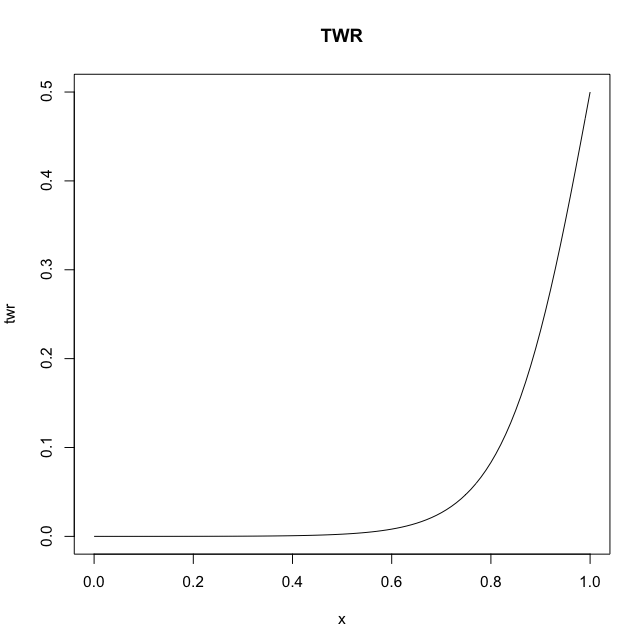
\includegraphics[scale=0.5]{twr_graph}
        \caption{Time Weighted Risk (TWR)}
        \label{figure:twr_graph}
    \end{center}
\end{figure}

\subsubsection{Example}
Given the repository represented in tables \ref{table:repo_files_commits} and
\ref{table:repo_commits}:

\begin{table}[H]
    \caption{Repository example -  files and commits}
    \label{table:repo_files_commits}
    \begin{center}
        \begin{tabular}{ | l | l | l | }
            \hline
            File & Commits \\ \hline
            main.java & A,B,C \\ \hline
            gui.java & A,D\\ \hline
            core.java & A  \\
            \hline
        \end{tabular}
    \end{center}
\end{table}

\begin{table}[H]
    \begin{center}
        \caption{Repository example - commits}
        \label{table:repo_commits}
        \begin{tabular}{ | l | l | l | }
            \hline
            Commit & Time & Bug fix? \\ \hline
            A & 5 & no \\ \hline
            B & 10 & no\\ \hline
            C & 15 & yes  \\ \hline
            D & 30 & yes  \\ \hline
        \end{tabular}
    \end{center}
\end{table}
Considering the current timestamp is 50 and the one of the beginning of the
repository is 5, the normalized timestamp for the bug-fixing commits are the
following:

\begin{equation}
ti_C = \frac{15 - 5}{50 - 5} = \frac{2}{9}\qquad
ti_D = \frac{30 - 5}{50 - 5} = \frac{5}{9}
\end{equation}

Using the previous timestamps, the scores for each file are:

\begin{equation}
Score_{main} \approx 0.000088 \qquad
Score_{gui} \approx 0.004805 \qquad
Score_{core} = 0
\end{equation}

Considering this model, the less reliable component is gui.java because it has
the highest score due the fact that exists a recent bug-fixing commit. If
someone asked you to find bugs in a repository you would do the same: inspecting
the files with the most commits related to bugs.

\subsubsection{Discussion}
TWR gives more importance to the most recent changes and that is a way of not
flagging old untouched files that developers do not want to fix. But, the
model is not complete enough because files that have score equal to zero may
have unfixed bugs. Therefore, these model should be improved with information
from others techniques.

Research has been done at Google where developers had the opportunity to choose
between this model and Fixcache (further discussed) and by seeing the results of
both of the algorithms, developers chose TWR, mainly because it considers the
most recent changes \cite{Chris2013}. The study revealed developers are
\"afraid\" of old source code so a model that highlights those old components
cannot be considered good.

\subsection{Fixcache and Bugcache}
Fixcache and Bugcache are defect prediction models based on cache and the
difference from other models is that they are more dynamic and have more
predictive power \cite{Kim:2007:PFC:1248820.1248881}. This models assume that
faults do not occur in isolation but in burst with other related faults.

A cache is a list of components where the granularity can be the executable
binary, module, file or method (entity). Since faults appear in bursts, the
cache is updated by the following policies:

\begin{itemize}
  \item new or modified files may have bugs (new and changed locality);
  \item buggy files can contain more bugs (temporal locality);
  \item files changed with buggy files may have bugs (spacial locality).
\end{itemize}

The size of the cache is fixed and when it is full, a policy of removal should
be chosen: the component to remove can be the least recent used (LRU), number
of recent changes, number of recent bugs and the number of authors. LRU is the
policy that performs better \cite{Sadowski2011}.

Fixcache updates the cache when the bug is fixed and Bugcache when the bug is
introduced. The bug-fixing changes are detected by mining the repository commits
and bugs database. Bug-introducing changes are detected by the bug-fixing
changes. For example, if file A has been fixed in a certain commit, the commit
that created this file is a bug-introducing change. Due the presence of false
positives, this technique can be improved by using bug databases.

A study concluded that Fixcache not only can do bug prediction in a certain
point of time but can predict with accuracy at weekly intervals
\cite{Sadowski2011}.

\subsection{Change Classification}
Change Classification model evaluates if a change will introduce a bug using
machine learning techniques by learning from previous bugs~\cite{Kim2008}. A
problem that may arise is the effect of noise in the training set, compromising
the recall and recognition of buggy changes, but techniques are available to
reduce this noise. The classifier decides if a change is buggy or clean with
78\% accuracy and 60\% percent bug recall on average~\cite{Kim2008}. This
technique has less prediction power but knowing that a commit introduced a
bug it is still useful. The main characteristics are:

\begin{itemize}
  \item classify changes at the file level as buggy or clean;
  \item detect when a bug is introduced and not when it is fixed;
  \item takes advantage of source code information (features);
  \item independent of the programming language using bag-of-words methods.
\end{itemize}

Support Vector Machines is the approach used to classify changes due its
performance in text classification applications. Change Classification can be
used as a commit checker, a bug indicator on source code editing and can change
the software engineering process by giving immediate feedback to trigger a code
inspection when a commit is made \cite{Kim2008}.

Some limitations are important to consider such as the process of extracting
features that depends how developers used Git and like other machine learning
approaches, it takes time to learn.

\section{Fault localization techniques}
Fault localization is the process of finding the component causing the software
execution deviating from its expected result. Traditionally, developers use
manual techniques just as injecting prints to debug values or breakpoints.
Automatic fault localization techniques are used to reduce the cost of finding
these faulty components.

\subsection{Program-spectra based}
Program-spectra based methods evaluates the probability of each component being
faulty by analyzing the program execution history \cite{Perez2004}. It is a
statistical technique that, for each test case, computes the spectrum, that is
the code coverage and execution result. The program spectrum is then the list
of test cases execution results and can be easily understood by the example in
table \ref{table:spectrum}.

\begin{table}[H]
    \begin{center}
    \caption{Program spectrum}
    \label{table:spectrum}
    \begin{tabular}{ | c | c | c | c | c | c |}
        \hline
        Test Case & Component A & Component B & Component C & Result \\ \hline
        T1 & X & & & Success \\ \hline
        T2 & X & X & & Failure \\ \hline
        T3 &  & X & & Failure \\ \hline
        T4 & X &  & X & Success \\ \hline
    \end{tabular}
    \end{center}
\end{table}

To determine what components are called in each test case it is used code
instrumentation. The program spectrum in table \ref{table:spectrum} use binary
flags so it is called hit spectra. From this input, the components that most
affects program execution are computed, calculating similarity coefficients
using the Ochiai formula \cite{Abreu:2009:SMF:1747491.1747511}. This technique
also exploits information from execution outcomes. The output is then the
similarity coefficient for each component, that is their likelihood of
containing the fault.

Spectrum Fault Localization (SFL) approaches have a good quality of diagnosis
and scale well, but is more accurate when the system have many test cases
\cite{Mayer2008}. There are some tools based on SFL such as:

\begin{description}
  \item[Gzoltar] \hfill \\
  An eclipse plugin\footnote{\url{http://gzoltar.com/}} that integrates with
  JUnit tests \cite{Campos:2012:GEP:2351676.2351752}.
  \item[Tarantula] \hfill \\
  A technique and a tool\footnote{\url{http://spideruci.org/fault-localization/}}
  that offers recommendations to reduce the time needed to find the fault
  \cite{jones05}.
\end{description}

\subsection{Model-based}
Model-based techniques use reasoning to do fault localization by having the
system knowledge a priori. The system model, the description of correct
behavior, is used to compare with the observed behavior of the program and then
the difference is used to identify components that explain this deviation
\cite{Mayer2008}. Since model-based approaches in software engineering require a
formal specification, to avoid this limitation the model is obtained by
inference from test cases \cite{Perez2004}. The type of model can be:

\begin{itemize}
  \item based on dependencies between program statements;
  \item based on computing values propagation;
  \item based on creating abstraction models for particular fault assumptions.
\end{itemize}

Model-based fault localization should be combined with others techniques since
the current approaches are not efficient, with high computational cost and scale
poorly.

\subsection{Barinel}
Barinel is a combination of Spectrum-based fault localization and Model Based
Diagnostic \cite{Abreu:2009:SMF:1747491.1747511}. It starts by receiving a
hit-spectra matrix, that contains the observation of running the test cases.

\newcommand{\pr}{\mbox{Pr}}
\newcommand{\likelihood}{\pr(obs_i, e_i \mid d)}
\newcommand{\gFunc}[1][d]{\displaystyle\prod_{j \in (d \cap obs_i)} g_j}

\begin{figure}[h]
  \begin{center}
    \begin{tabular}{c|ccc|c}
    	& \multicolumn{3}{|c|}{$obs$} &      \\
      & $c_1$ & $c_2$ & $c_3$ & e     \\ \hline
      $t_1$ & 1     & 1     & 0     & 1     \\
      $t_2$ & 0     & 1     & 1     & 1     \\
      $t_3$ & 1     & 0     & 0     & 1     \\
      $t_4$ & 1     & 0     & 1     & 0     \\
    \end{tabular}
  \end{center}
  \caption{Hit-spectra matrix example}
  \label{figure:hit_spectra}
\end{figure}

Figure \ref{figure:hit_spectra} shows an example of a hit-spectra matrix, with
the outcome $e$ of every test case $t$ and the components involved. For example,
test case $t_1$ hits components $\{c_1, c_2\}$ and fails.

The algorithm then takes the following steps:
\begin{description}

\item[Candidate generation] \hfill \\
Only minimal candidates are generated. A candidate \( d \) is a set of
components that explains the observed behaviour of the program. In this example,
the list of candidates are:
\begin{itemize}
\item \( d_1 = \{c_1, c_2\} \)
\item \( d_2 = \{c_1, c_3\} \)
\end{itemize}

\item[Candidate ranking] \hfill \\
Each candidate \( d \)  is evaluated by computing the posterior probability
using the Na\"ive Bayes rule:

\begin{equation}
	\pr(d\mid obs,e) =  \pr(d) \cdot \prod_{i}\frac{\likelihood}{\pr(obs_i)}
\end{equation}

The denominator $\pr(obs_i)$ is a term that is normalized for all candidates
and it is not used for ranking. Let \( p_j\) denote the prior probability of a
component being faulty. Then, the prior  $\pr(d)$  of a candidate $d$ is:

\begin{equation}
  \pr(d) = \prod_{j \in d} p_j \cdot \prod_{j \notin d} (1 - p_j)
\end{equation}

Let $g_j$ denote the probability of a component behaving normally (goodness).
Then $\pr(obs_i,e_i \mid d)$ is computed by:

\begin{equation}\label{eq:likelihood_func}
  \pr(obs_i, e_i \mid  d) =
  \begin{cases}
    \gFunc     & \textrm{if   } e_i = 0 \\
	1 - \gFunc & \textrm{otherwise}
  \end{cases}
\end{equation}

If for a certain component $g_j$ is not available, it is computed by maximizing
$\pr(obs,e \mid d)$ (Maximum Likelihood Estimation (MLE)), for the Na\"ive Bayes
classifier. Considering our example, the probabilities for both candidates $d_1$
and $d_2$ are:

\begin{equation}
    \pr(d_1 \mid obs,e) =
    \overbrace{\bigg(\frac{1}{1000} \cdot \frac{1}{1000} \cdot \bigg(1 - \frac{1}{1000}\bigg)\bigg)}^{\pr(d)}
    \times
    \overbrace{
      \underbrace{(1-g_1 \cdot g_2)}_{t_1}
      \times
      \underbrace{(1-g_2)}_{t_2}
      \times
      \underbrace{(1-g_1)}_{t_3}
      \times
      \underbrace{g_1}_{t_4}
    }^{\pr(obs,e \mid d)}
\end{equation}
%
\begin{equation}
    \pr(d_2 \mid obs,e) =
    \overbrace{\bigg(\frac{1}{1000} \cdot \frac{1}{1000} \cdot \bigg(1 - \frac{1}{1000}\bigg)\bigg)}^{\pr(d)}
    \times
    \overbrace{
      \underbrace{(1-g_1)}_{t_1}
      \times
      \underbrace{(1-g_3)}_{t_2}
      \times
      \underbrace{(1-g_1)}_{t_3}
      \times
      \underbrace{g_1 \cdot g_3}_{t_4}
    }^{\pr(obs,e \mid d)}
\end{equation}
\end{description}

By performing MLE for both functions:
\begin{itemize}
\item $\pr(d_1 \mid obs,e)$ is maximized for $g_1=0.47$ and $g_2=0.19$;
\item $\pr(d_2 \mid obs,e)$ is maximized for $g_1=0.41$ and $g_3=0.50$.
\end{itemize}

Applying the computed values for goodness, $\pr(d_1 \mid obs,e)=1.9 \times
10^{-9}$ and $\pr(d_2 \mid obs,e)=4.0 \times 10^{-10}$. The ranking is then
$(d_1,d_2)$.


\subsection{Crowbar}
Crowbar\footnote{\url{https://crowbar.io}}, formerly known as Gzoltar, is a tool
for Java projects that relies on test cases (dynamic analysis) to help
developers locate where is the fault of a bug. It uses the Barinel algorithm,
combining Spectrum-Based Fault Localization and Model-Based approaches. It
supports granularity until the statement level and use code instrumentation by
injecting probes in the source code.

\begin{figure}[H]
    \begin{center}
        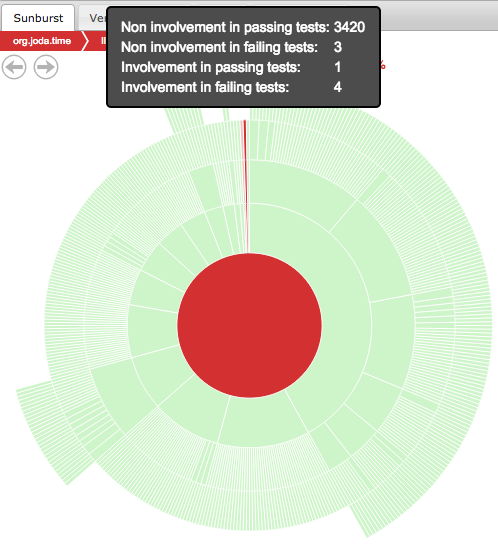
\includegraphics[scale=0.5]{crowbar}
        \caption{Crowbar sunburst chart report}
        \label{figure:crowbar_report}
    \end{center}
\end{figure}

Figure \ref{figure:crowbar_report} shows an example of a sunburst report that
can be zoomed. In this type of visualization, the granularity of components
increases from the center to the exterior (statement) and the colors are a clue
to find faulty components. We also have the possibility to visualize the report
as a vertical partition.

\subsubsection*{Usage}
Crowbar supports Junit\footnote{\url{http://junit.org/}} and
TestNG\footnote{\url{http://testng.org/}}. It runs as a Java agent on the test
suite through the Maven\footnote{\url{https://maven.apache.org/}} Surefire
Plugin\footnote{\url{https://maven.apache.org/surefire/maven-surefire-plugin/}}.
Configuration is done in the file pom.xml\footnote{\url{https://maven.apache.org/guides/introduction/introduction-to-the-pom.html}},
that contains information for Maven about the project and configuration details
to build and test.

Crowbar will then display the results on a web server by displaying an URL that
we must access on a browser to be able to see the report.

\section{Similar tools}
There are plenty of tools available that analyse Software projects. They
evaluate code quality and warn developers about problems detected.

\subsection{Codacy}

Codacy \footnote{\url{https://codacy.com}} is an automatic software revision
service (static analysis) that uses defect prediction models to estimate
software component reliability. It is a Startup based in Lisbon that won the
best pitch award in 2014 Web Summit in London and it is available with free
(Open Source) and paid plans.

This service uses the Change Classification principle, classifying a commit as
buggy or clean. It supports Scala, Javascript, Python, PHP and CSS. With a few
steps it is possible connecting our repository, hosted at Bitbucket or Github.

\begin{figure}[H]
    \begin{center}
        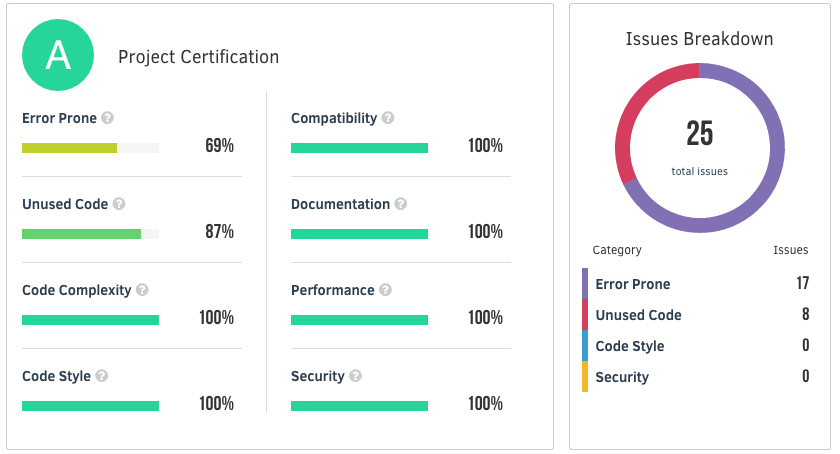
\includegraphics[width=\textwidth]{codacy-report}
        \caption{Codacy dashboard}
        \label{figure:codacy_dashboard}
    \end{center}
\end{figure}

Figure \ref{figure:codacy_dashboard} shows the dashboard with a variety of
metrics, reporting a score for code style, errors, code complexity, performance,
unused code, compatibility, etc. New and fixed issues are presented, therefore,
developers feel rewarded and motivated to improve code quality, a feature that
somehow failed in the tool developed in a research conducted at Google in 2013
by Chris Lewis et al. \cite{Chris2013}.

\subsection{Moskito}
Moskito\footnote{\url{http://moskito.org}} is a tool that monitors Java Web
applications, does fault localization and it is free and Open Source~\footnote{\url{https://github.com/anotheria/moskito-control}}.
Developers must use annotations to declare what classes or methods to monitor
and it does not require changing code, which make this solution simple to use.
Two main elements of this tool are the agent and server, where the first
collects data and sends it to the server, that processes and displays
information in a dashboard.

\begin{lstlisting}[language=java, caption=Usage example from Moskito documentation]
//simply add @Monitor
@Monitor
public class MonitoredClass {
    public void firstMethod(){
        //do something
    }
    public void secondMethod(){
        //do something else
    }
    //you can also exclude methods from monitoring:
    @DontMonitor
    public void doNotMonitorMe(){
    }
}
\end{lstlisting}

\begin{figure}[H]
    \begin{center}
        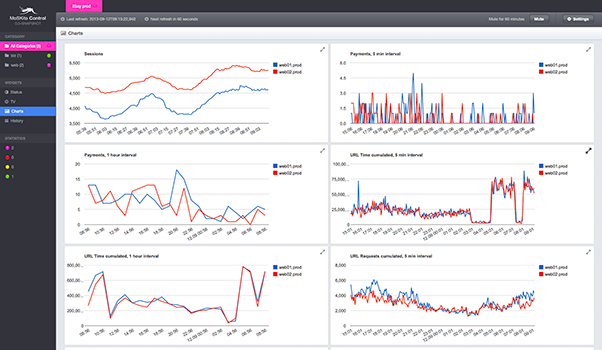
\includegraphics[scale=0.5]{moskito-control}
        \caption{Moskito dashboard}
        \label{figure:moskito_dashboard}
    \end{center}
\end{figure}

The dashboard at figure \ref{figure:moskito_dashboard} displays performance
charts taken from multiple nodes. When a component performance changes, the
health indicator change its color, so developers can fix the problem
immediately, before affecting the whole application and users complain.

\subsection{SensioLabsInsight}
SensioLabsInsight in figure \ref{figure:sensiolabsinsight}, is a web service
\footnote{\url{https://insight.sensiolabs.com/}} that continuously analyzes PHP
projects in terms of security, bugs and other quality checks. It also does
dynamic analysis to improve diagnostic accuracy. Integrates with Github and
Bitbucket services and is free for Open Source projects.

\begin{figure}[H]
    \begin{center}
        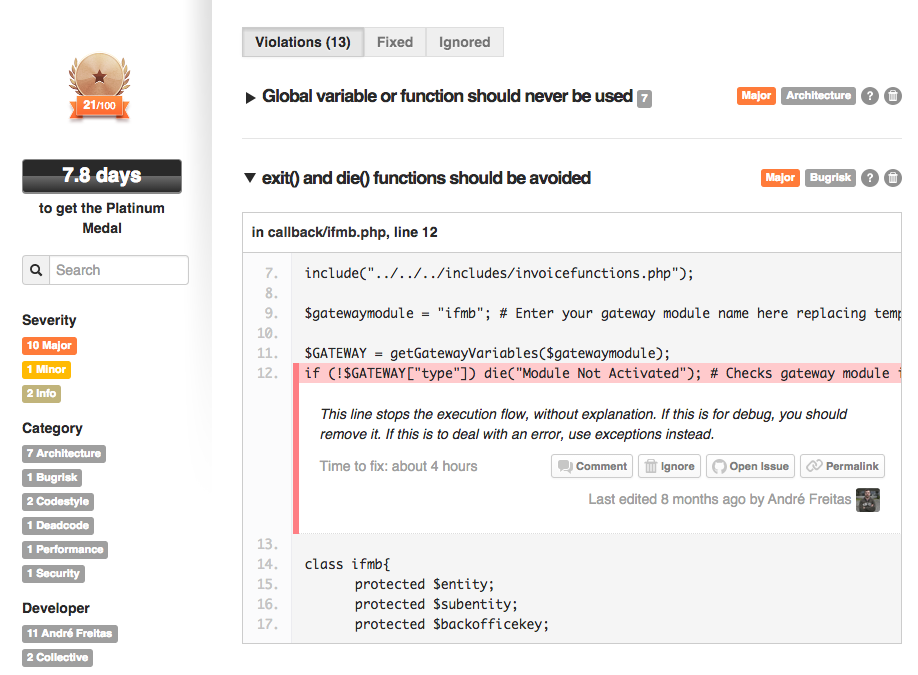
\includegraphics[scale=0.4]{sensiolabsinsight}
        \caption{Example of a report from SensioLabsInsight}
        \label{figure:sensiolabsinsight}
    \end{center}
\end{figure}

\subsection{Code Climate}
Code Climate \footnote{\url{https://codeclimate.com/}} in figure
\ref{figure:codeclimate}, is another service that analyzes PHP, Python,
Javascript and Ruby using static analysis. It essentially produce warnings about
issues in code complexity, duplication, style and readability. Also displays
insights about churn (lines changed) versus code quality. The dashboard is very
complete since we can check listed issues or inspect code along with the
warnings produced. It has a free plan for Open Source projects.

\begin{figure}[H]
    \begin{center}
        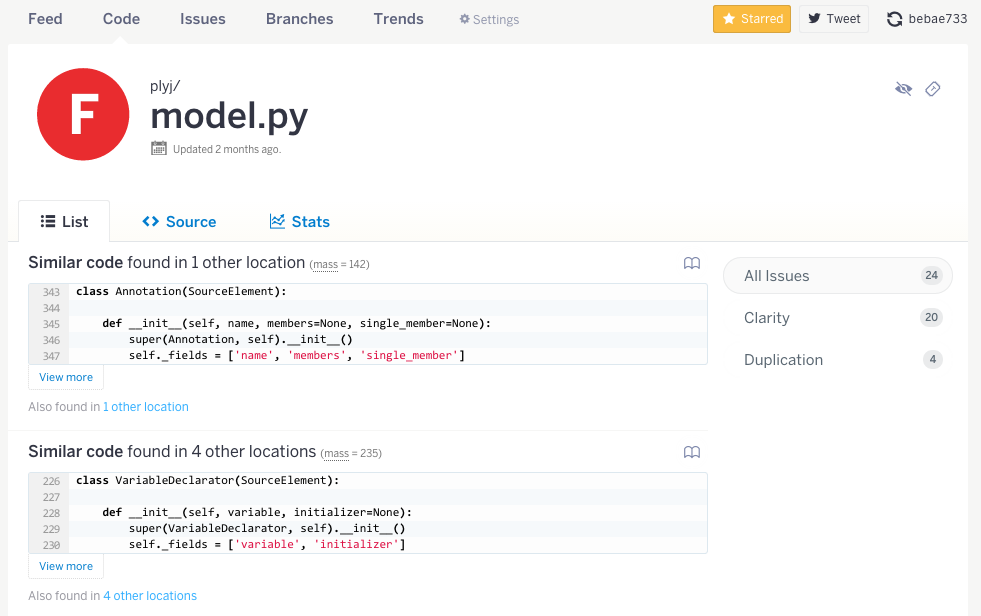
\includegraphics[scale=0.4]{codeclimate}
        \caption{Issues listed on Code Climate}
        \label{figure:codeclimate}
    \end{center}
\end{figure}

\subsection{Pull Review}
Pull Review \footnote{\url{https://pullreview.com/}} in figure
\ref{figure:pullreview}, is an automatic code review service (static analysis)
just for Ruby. It gives feedback for style, duplication, code smells,
documentation, security and tests. It has the ability of linking a Github,
Gitlab or Bitbucket repository and is also free for Open Source.

\begin{figure}[H]
    \begin{center}
        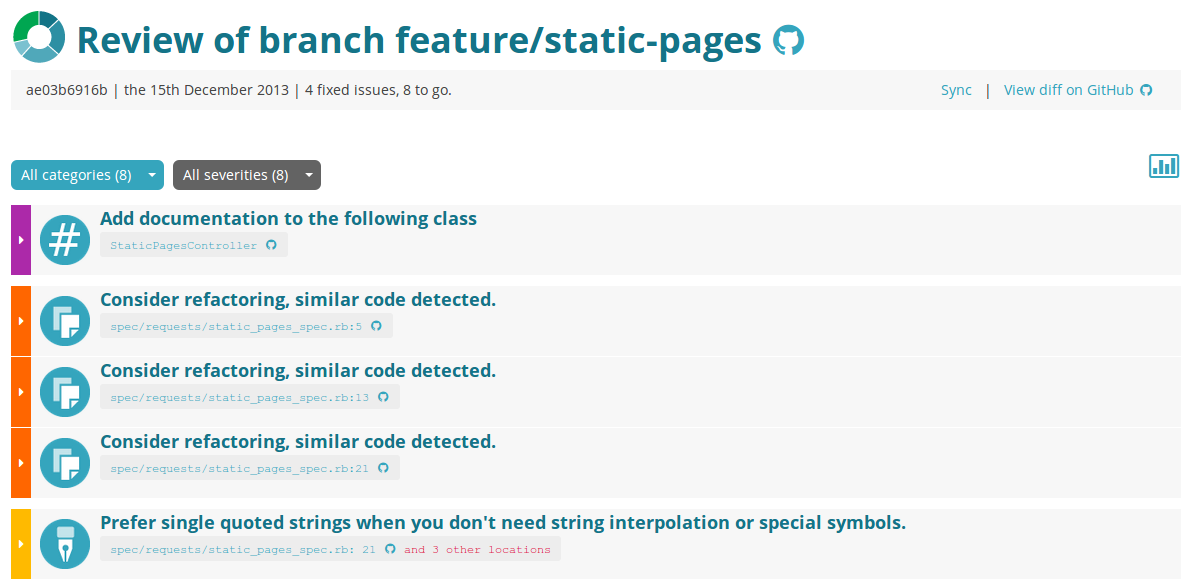
\includegraphics[scale=0.3]{pullreview}
        \caption{Pull Review report}
        \label{figure:pullreview}
    \end{center}
\end{figure}

\chapter{A Technique to Estimate Defect Probabilities} \label{chap:methods}

\section*{}
In this chapter it is discussed the methodologies used to answer the research
 questions.

\section{Schwa}
Schwa is the tool developed for research. Source code is available at
Github\footnote{\url{https://github.com/andrefreitas/schwa}} as an Open Source
project under MIT 2.0 license. It was developed in Python and is hosted at
PyPi\footnote{\url{https://pypi.python.org/pypi/Schwa}}, the Python Package
Index.

\subsection{Installation}
Schwa relies on Python 3 and Git and they are the only dependencies. Can be
easily installed using pip
\footnote{\url{https://pip.pypa.io/en/latest/installing.html}}.

\begin{lstlisting}[language=bash, caption=Schwa installation command]
   pip3 install schwa --pre
\end{lstlisting}

\subsection{Usage}
It can be used as a command line tool and imported as a Python package.
An example of running Schwa, is analyzing the last 20 commits of the Joda Time
repository:

\begin{lstlisting}[language=bash, caption=Running Schwa on Joda Time]
  schwa git/joda-time --commits 20
\end{lstlisting}

\subsection{Visualization}

\begin{figure}[H]
    \begin{center}
        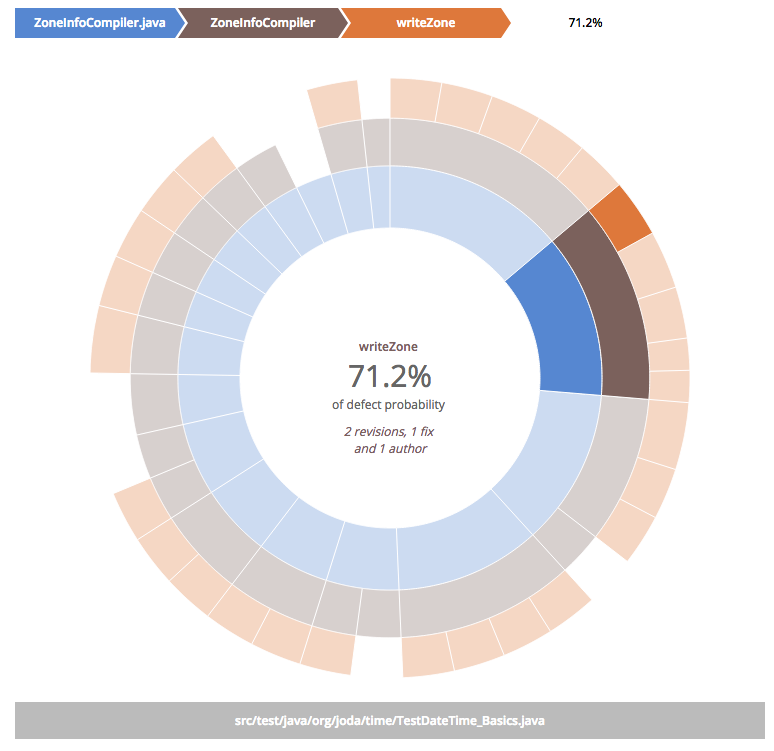
\includegraphics[scale=0.5]{schwa-sunburst}
        \caption{Sunburst results for Joda Time}
        \label{figure:sunburst-joda}
    \end{center}
\end{figure}

The report is launched in a browser and is displayed in a Sunburst chart,
described in Figure \ref{figure:sunburst-joda}, that is a simple way of showing
a hierarchy of results. It is inspired from the visualization style of Crowbar.
Granularity of components increases from the center to the periphery and the
longer the arc, the higher the probability of defect. Blue nodes are files,
brown are classes and orange are methods. The path of selected files are
displayed in the bottom.

This visualization also gives some reasoning about the defect probability,
displaying the values for revisions, fixes and authors.

\subsection{Process}
Mining a Software repository can be essentially divided in two phases:
Extraction and Analysis. The rationale is that first we only extract the most
important information and then extracted data is analyzed. By using a generic
representation of a repository as the input for the analysis, Schwa can be
extended with more SCM tools, such as Mercurial and Apache Subversion. The
process pipeline is described in figure \ref{figure:schwa_process}.

\begin{figure}[H]
    \begin{center}
        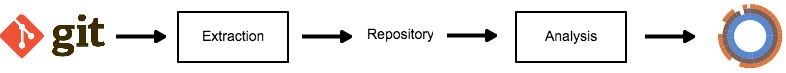
\includegraphics[scale=0.5]{process}
        \caption{Process pipeline}
        \label{figure:schwa_process}
    \end{center}
\end{figure}

\subsubsection{Extraction}
Extraction is the phase that takes more time due the amount of I/O operations
reading blobs, even with code parallelization. Considering these performance
issues, Schwa iterates over commits, so it is possible to just extract for
example, the last 10 commits. For each commit every
change is parsed so the most important information is:

\begin{itemize}
\item  \textbf{Message} Commit message that is used to evaluate if the commit
is fixing a bug;
\item  \textbf{Author} Commit author's email to track the number of contributors
a component had;
\item  \textbf{Timestamp} An integer with the Unix Timestamp, used to track
changes in components and achieving time relevance (TWR), that is distinguishing
 recently changed components from old components;
\item  \textbf{Diffs} The list of commit changes in components, such as files,
classes and methods.
\end{itemize}

Schwa extracts data from Git repositories using the GitPython
library\footnote{\url{https://github.com/gitpython-developers/GitPython}}. For
Java source files we track changes until the method granularity. For other
programming languages we only track changes until the file granularity.

Parsing Java is possible by using the
Plyj\footnote{\url{https://github.com/musiKk/plyj}} library, that has been
modified to include line information for Classes and Methods in the Abstract
Syntax Tree.

When the extraction finishes, all the important information has been collected
and is represented in the model of figure \ref{figure:repository_model}.

\begin{figure}[H]
    \begin{center}
        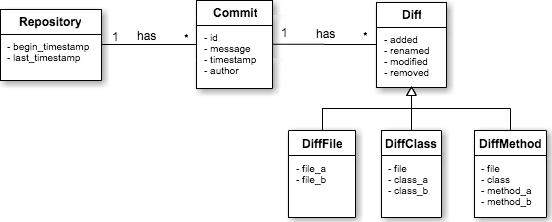
\includegraphics[scale=0.6]{Repository}
        \caption{Repository Model}
        \label{figure:repository_model}
    \end{center}
\end{figure}

Begin and last timestamps in the Repository class are referring to the first and
last commits and are necessary for the TWR formula. Diffs have been divided in
subclasses for each granularity. A diff is a result of changing a version A
resulting in another version B. To make more clear this concept, consider the
following patch:

\begin{lstlisting}[language=java, caption=Patch in API.java]
class API {
  static void login(String email, String password,
  AsyncHttpResponseHandler responseHandler){
      RequestParams params = new RequestParams();
      params.put("email", email);
      params.put("password", password);
+     params.put("token", "j76g367f4");
      client.post(url + "/login", params, responseHandler);
  }

+  static void getShows(AsyncHttpResponseHandler responseHandler) {
+   client.get(url + "/shows", responseHandler);
+  }

-  static void getUsers(AsyncHttpResponseHandler responseHandler) {
-   client.get(url + "/users", responseHandler);
-  }
}
\end{lstlisting}


The list of diffs instances would be:

\begin{lstlisting}[language=python, caption=List of Diff instances]
DiffFile(file_a="API.java", file_b="API.java", modified=True)
DiffClass(file_name="API.java", class_a="API", class_b="API", modified=True)
DiffMethod("API.java", class_name="API", method_a="login", method_b="login", modified=True)
DiffMethod("API.java", class_name="API", method_b="getShows", added=True)
DiffMethod("API.java", class_name="API", method_a="getUsers", removed=True)
\end{lstlisting}

We are currently supporting only renaming of files since detecting a renaming of
a Class or Method can be subjective. For example, it is not trivial by parsing
a patch, recognizing the difference of deleting and creating a new method with
the same body or only changing the method signature.

\subsubsection{Analysis}
Analysis receives a Repository (figure \ref{figure:repository_model}) as the
input and will iterate again over commits but now with the objective of
tracking the following metrics:

\begin{itemize}
\item \textbf{Revisions} The more a component had recently new changes, the
higher will be revisions score. Graves \textit{et al.} showed that revisions is
 a predictive variable \cite{859533};
\item \textbf{Fixes} The more a component had recently new bug-fixes, the higher
will be fixes score; Zimmerman \textit{et al.} showed that past defects have the
highest correlation with future defects \cite{Zimmermann:2007:PDE:1268984.1269057};
\item \textbf{Authors} The more a component had recently new authors, the higher
will be authors score. Authors is a process metric that can be also used to
predict defects \cite{Moser:2008:CAE:1368088.1368114,D'Ambros:2012:EDP:2318097.2318149}.
\end{itemize}

Metrics are tracked the same way for any granularity and they were selected
after a revision of the state of the art in MSR.
Considering our goal of improving Crowbar fault localization results, the
Time-Weighted Risk approach is the one that fits this scenario, since it is a
rank-based technique. TWR is not only used only for Fixes but also for Revisions
and Authors, since they can benefit of time relevance, something that was not
possible when using counters.

We also found that the TWR curve in the Figure \ref{figure:twr_graph}, should be
modified, because even recently changed components were having low score. The
problem, is that when \( t_i <= 0.8 \), TWR is low. We want the curve to start
growing sooner so therefore we modified the TWR equation with the Time Range
(TR) parameter, resulting in a new expression:

\begin{equation}
twr(t_i) = \frac{1}{1 + e^{-12t_i + 2 + ( (1 - TR)* 10) }}
\end{equation}

TR varies from 0 to 1 . In figure \ref{figure:twr_modified_graph} with TR = 0.5,
the curve goes to the left giving more score to older timestamps and increasing
the score of $t_i = 1.0$ to 1.0.

\begin{figure}[!ht]
    \begin{center}
        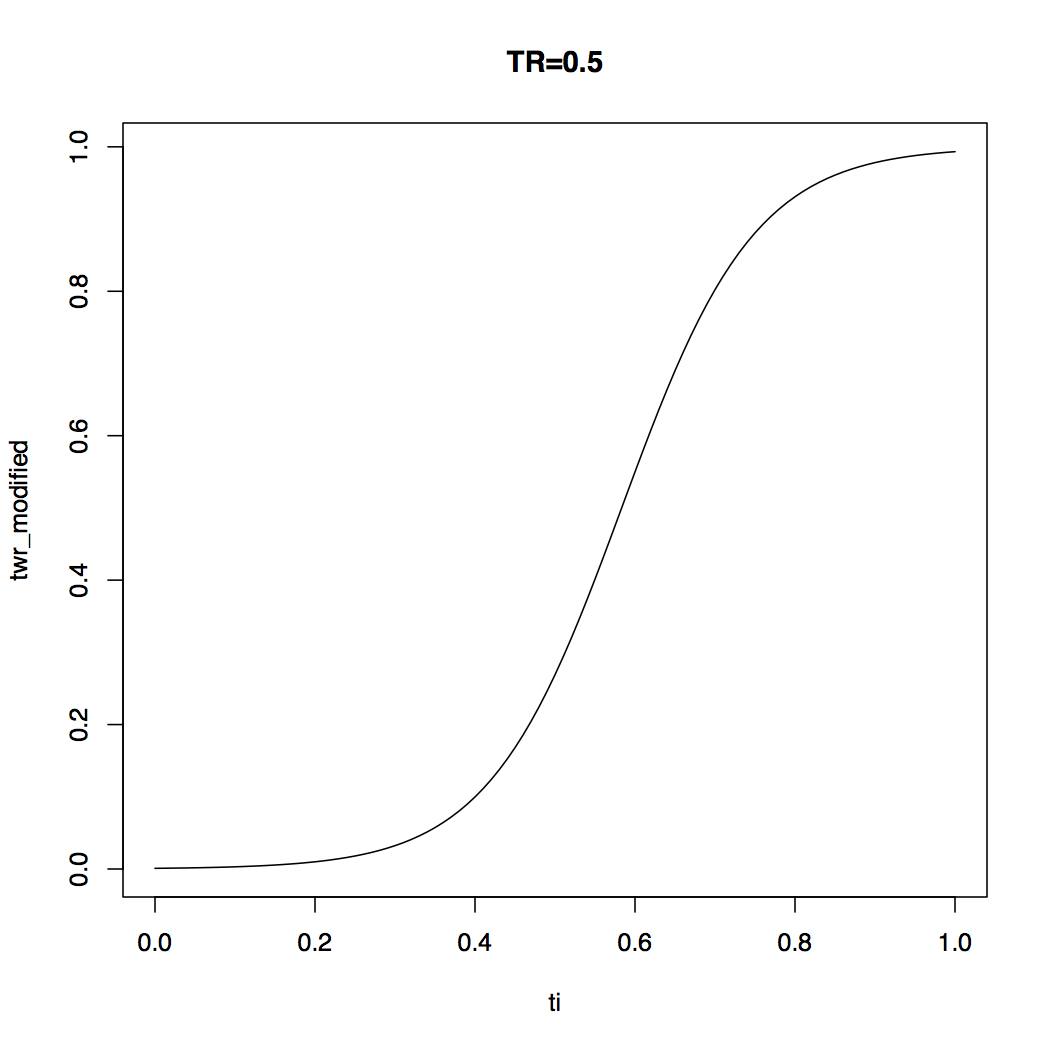
\includegraphics[scale=0.5]{twr_modified_graph}
        \caption{Modified Time Weighted Risk (TWR)}
        \label{figure:twr_modified_graph}
    \end{center}
\end{figure}

With a deeper understanding about how TWR works, algorithm
\ref{algorithm:analysis} describes the steps involved in the analysis, in a
simplified way.\*

\begin{algorithm}[H]
\For{each commit in the repository}{
  twr = compute twr

  \For{each component in the commit}{
    component.revisions += twr

    \If{commit is bug fix}{
        component.fixes += twr
    }

    \If{is new author}{
        component.authors += twr
    }
  }
}
\caption{Analysis algorithm}
\label{algorithm:analysis}
\end{algorithm}

We detect if a commit is fixing a bug by searching for keywords in the message.
Since Github\footnote{\url{http://github.com}} is the most used Git repository
hosting service, the regular expression was based on Github's syntax for
closing issues by commit messages
\footnote{\url{https://help.github.com/articles/closing-issues-via-commit-messages/}}.
The regular expression is the following:
\\
\\
\begin{lstlisting}[language=python, caption=Bug-fixing message regular expression]
fix(e[ds])?|bugs?|defects?|patch|close([sd])?|resolve([sd])?
\end{lstlisting}

\subsubsection{Defect prediction computation}
When the analysis is finished, Schwa computes the defect probability for every
component by doing a weighted average of the metrics:

\begin{equation}
score = revisions * revisions_{weight} + fixes * fixes_{weight} + authors * authors_{weight}
\end{equation}

Then the score is normalized to a value from 0 to 1, that is the estimation of
the defect probability:

\begin{equation}
defect_{probability} = 1 - e^{-score}
\end{equation}

By default, Schwa uses the weights: 0.25 for revisions, 0.25 for authors and 0.5
for fixes. These weights are based from the existing research in MSR
\cite{859533, Zimmermann:2007:PDE:1268984.1269057, Moser:2008:CAE:1368088.1368114,D'Ambros:2012:EDP:2318097.2318149}.
They may be different for each type of software project. For example, in a
project with a lot of contributors, tracking authors can be important, but in a
project with just a contributor, this metric is not relevant because the number
of authors never changes.

\section{Features weight estimation}
Estimating the weights of each feature: revisions, fixes and authors is an
optimization problem. Our approach was using Genetic Algorithms for searching
the best solution and encoding individuals as:

\begin{equation}
\{R, F, A\}
\end{equation}

$R$, $F$ and $A$ are the weights from 0 to 1 for revisions, fixes and authors,
respectively. They have been encoded to binary with 3 bits of precision, that
means that we can represent \( 2 ^3 = 8 \) different values for each feature.
Increasing bits precision has the cost of decreasing performance.

The fitness function \ref{eq:fitness_ga} is the sum of the distance between
involved and not involved components for every bug-fixing commit \(m\) with a
penalty for invalid solutions: weights cannot be 0 and their sum must be 1. This
rationale results in the following expressions:

\begin{equation}
\label{eq:fitness_ga}
fitness(R,F,A) =
  \begin{cases}
      \hfill \sum_{m \in commits_{bugfixing}}^{} distance(R,F,A,m)  \hfill & \text{ if constraints($R$,$F$,$A$)}\\
      \hfill -\infty \hfill & \text{ otherwise} \\
  \end{cases}
\end{equation}

\begin{equation}
constraints(R,F,A) = (R+F+A) == 1 \wedge (R*F*A) > 0
\end{equation}

\begin{equation}
distance(R,F,A,m) = \frac{ \sum_{c \in involved(m)}^{} score(R,F,A,c) }{|involved(m)|} - \frac{ \sum_{c \in (Components \setminus involved(m))}^{} score(R,F,A,c) }{|(Components \setminus involved(m))|}
\end{equation}

\begin{equation}
score(R,F,A,c) = c_{revisions} * R + c_{fixes} * F + c_{authors} * A
\end{equation}

This means that in bug-introducing commits, faulty components should have
higher score than non faulty components. Besides finding features weights,
this approach helps us validate if Schwa is predicting defects correctly. Due
to performance constraints, the fitness function only evaluates components at the
file granularity. Note that this granularity is only for Schwa learning mode. For
defect prediction, Schwa still operates with method granularity for Java.


\section{Diagnostic cost}
Crowbar outputs a rank of components ordered by their probability of having the
fault. To measure the quality of this diagnostic, the heuristic used is Diagnostic
Cost \cite{6693085} that is the average of the minimum and maximum distance that
faulty components are from the top of the rank. For multiple faults, this cost
is computed considering the lowest faulty component.

\begin{equation}
diagnostic_{cost} = \frac{min_{distance} + max_{distance} - |faulty|}{2}
\end{equation}

\subsection{Example}
\( C_2 \) is the component that have the fault.

\begin{table}[h]
\centering
\caption{Examples of ranks}
\label{my-label}
\begin{tabular}{|c|c|c|}
\hline
Position & Rank 1 & Rank 2 \\ \hline
    1    &   \( C_3(0.234) \)   &  \( *C_2(0.500) \)     \\ \hline
    2    &   \( C_5(0.145) \)   &  \( C_5(0.120) \)     \\ \hline
    3    &   \( *C_2(0.145) \)   &  \( C_3(0.120) \)   \\ \hline
    Diagnostic Cost   &   1   &  0  \\ \hline
\end{tabular}
\end{table}

In Rank 1 \(C_5\) and \(C_2\) components have the same probability so \(C_2\)
position can be 2 or 3 depending on the result of ordering the rank. In Rank 2
\(C_2\)  is on the first position so the cost is 0.

\subsection{Schwa integration with Crowbar}
By using Schwa, the goal is improving Barinel results, reducing the Diagnostic
Cost by evaluating if defect probabilities should be used in priors ($p_j$),
goodness ($g_j$) or both parameters. In Barinel the meaning of these parameters
is the following:

\begin{description}
\item[Prior] \hfill \\
The probability a component have of causing an error and is by default
\( \frac{1}{1000} \), based on the heuristic that for every 1000 lines of code
heuristic there is one bug.
\item[Goodness] \hfill \\
The probability of a component behaving normally and by default is computed by
using the Maximum Likelihood Estimation that is heavy to compute. By default is $0.5$.
\end{description}

If the defect probability of Schwa is used for goodness, it is computed by:
\begin{equation}
\pr(obs_i,e_i \mid d) = 1 - defect_{probability}(c)
\end{equation}

\chapter{Experimental results} \label{chap:results}

\section*{}
This chapter provides the results of the experiments conducted. The setup and
configurations are also described. There is a public page with the experimental
results of Schwa on Github \footnote{\url{https://github.com/andrefreitas/schwa/wiki/Experiments}}.

\section{Features weight estimation}
In this section we present the results of learning the features weights, that is
the importance of each of them, when computing the defect probability.

\subsection{Experimental setup}
To run this experiment, Schwa was invoked in the learning mode with 5, 50 and
100 commits with the script in listing 4.1. The version of Schwa used was
0.1.dev24(tagged on Git).

Running genetic algorithms takes a substantial time of computation, so we have
used Crowdsourcing to run the experiment in a variety of projects. We collected
data from academic, enterprise and Open Source projects to have results from
different contexts.

\begin{lstlisting}[language=bash, caption=Shell script used to learn features weights]
if [ -z "$1" ]
then
  echo "usage: $0 <git repository path>"
else
  touch report_$USER.txt
  echo "This will take a while..."
  echo "Learning with 5 commits"
  schwa $1 --commits 5 -l >> report_$USER.txt
  echo "Learning with 50 commits"
  schwa $1 --commits 50 -l >> report_$USER.txt
  echo "Learning with 100 commits"
  schwa $1 --commits 100 -l >> report_$USER.txt
  echo "Thank you! You are the best! Send report_$USER.txt to Andre :)"
fi
\end{lstlisting}

\subsection{Results}
Here we show the results for each repository. In the following tables, in each
row we have the maximum number of commits, the weights of revisions, fixes and
authors and the fitness value. The main objective of these tables is providing
the importance of each feature for a certain project.

\subsubsection{Schwa}
The experiment was run in
Schwa\footnote{\url{https://github.com/andrefreitas/schwa}} itself, that have
only one contributor. It is developed mostly with Python along with HTML, CSS
and Javascript.

\begin{table}[H]
    \centering
    \caption{Schwa results}
    \label{table:learning_schwa}
    \begin{tabular}{|l|l|l|l|l|}
        \hline
        Commits & Revisions & Fixes & Authors & Fitness \\ \hline
        5 & 0.2857 & 0.2857 & 0.4286 & 0 \\ \hline
        50 & 0.7143 & 0.1429 & 0.1429 & 1.0699 \\ \hline
        100 & 0.7143 & 0.1429 & 0.1429 & 1.1875 \\ \hline
    \end{tabular}
\end{table}

For 5 commits, the fitness function is 0, so it is not possible to estimate
correctly the weights. For 50 and 100 commits, revisions is the most important
feature.

\subsubsection{Libcrowbar}
Libcrowbar is the main repository of Crowbar and have multiple academic
contributors. The technologies used are Java, C++, HTML, CSS and Javascript.

\begin{table}[H]
    \centering
    \caption{Libcrowbar results}
    \label{table:learning_libcrowbar}
    \begin{tabular}{|l|l|l|l|l|}
        \hline
        Commits & Revisions & Fixes & Authors & Fitness \\ \hline
        5 & 0.1429 & 0.1429 & 0.7143 & 0.3486 \\ \hline
        50 & 0.7143 & 0.1429 & 0.1429 & 1.3639 \\ \hline
        100 & 0.7143 & 0.1429 & 0.1429 & 0.3387 \\ \hline
    \end{tabular}
\end{table}
For the last 5 commits, authors is the most important feature and for 50 and 100
commits, is revisions.

\subsubsection{Joda Time}
Joda Time\footnote{\url{https://github.com/JodaOrg/joda-time}} is an Open Source
time library for Java with multiple contributors.

\begin{table}[H]
    \centering
    \caption{Joda Time results}
    \label{table:learning_jodatime}
    \begin{tabular}{|l|l|l|l|l|}
        \hline
        Commits & Revisions & Fixes & Authors & Fitness \\ \hline
        5 & 0.1429 & 0.2857 & 0.5714 & 0 \\ \hline
        50 & 0.1429 & 0.7143 & 0.1429 & -2.1874 \\ \hline
        100 & 0.1429 & 0.7143 & 0.1429 & 0.3893 \\ \hline
    \end{tabular}
\end{table}
For this project only for 100 commits the fitness function is > 0, showing that
fixes is the most important feature.

\subsubsection{Meo Arena}
Meo Arena\footnote{\url{https://bitbucket.org/andrefreitas/feup-cmov-meoarena/}}
is a mobile application developed for Android in an academic context with two
contributors. It relies on Java and Python.

\begin{table}[H]
    \centering
    \caption{Meo Arena results}
    \label{table:learning_meoarena}
    \begin{tabular}{|l|l|l|l|l|}
        \hline
        Commits & Revisions & Fixes & Authors & Fitness \\ \hline
        5 & 0.2857 & 0.4286 & 0.2857 & 0 \\ \hline
        50 & 0.7143 & 0.1429 & 0.1429 & 1.6712 \\ \hline
        100 & 0.7143 & 0.1429 & 0.1429 & 0.7368 \\ \hline
    \end{tabular}
\end{table}

For 5 commits, fitness is equal to zero. For 50 and 100 commits the most
important feature is revisions.

\subsubsection{Mongo Java Driver}
Mongo Java driver\footnote{\url{https://github.com/mongodb/mongo-java-driver}}
is an Open Source projects and enables Java applications to communicate with a
MongoDB server. It is developed with Java and Groovy and has multiple
contributors.

\begin{table}[H]
    \centering
    \caption{Mongo Java driver results}
    \label{table:learning_mongojavadriver}
    \begin{tabular}{|l|l|l|l|l|}
        \hline
        Commits & Revisions & Fixes & Authors & Fitness \\ \hline
        5 & 0.7143 & 0.1429 & 0.1429 & 0.3486 \\ \hline
        50 & 0.7143 & 0.1429 & 0.1429 & 0.1685 \\ \hline
        100 & 0.1429 & 0.7143  & 0.1429 & 1.4666 \\ \hline
    \end{tabular}
\end{table}

For 5 and 50 commits the most important feature is revisions but for 100, is
fixes.

\subsubsection{Scraim}
Scraim\footnote{\url{https://scraim.com/}} is a web-based project management
tool developed by the company Strongstep. It is build on top of Redmine and
uses Ruby on Rails.

\begin{table}[H]
    \centering
    \caption{Scraim results}
    \label{table:learning_scraim}
    \begin{tabular}{|l|l|l|l|l|}
        \hline
        Commits & Revisions & Fixes & Authors & Fitness \\ \hline
        5         & 0.4286     & 0.1429 & 0.4286   & 0.3486 \\ \hline
        50        & 0.1429 & 0.1429 & 0.7143   & 0.3146 \\ \hline
        100       & 0.1429     & 0.7143  & 0.1429    & 0.9399 \\ \hline
    \end{tabular}
\end{table}
For 5 commits, revisions and authors are both important. For 50, authors is the
most important and for 100 is fixes.

\subsubsection{Trainsim}
Trainsim is an academic project developed with Java and Swing with one
contributor.

\begin{table}[H]
    \centering
    \caption{Trainsim results}
    \label{table:learning_trainsim}
    \begin{tabular}{|l|l|l|l|l|}
        \hline
        Commits & Revisions & Fixes & Authors & Fitness \\ \hline
        5         & 0.1429     & 0.7143 & 0.1429   & 0 \\ \hline
        50        & 0.7143 & 0.1429 & 0.1429   & 1.5945 \\ \hline
        100       & 0.5714     & 0.2857  & 0.1429    & 2.0425 \\ \hline
    \end{tabular}
\end{table}

For 5 commits fitness is zero, for 50 and 100 the most important is revisions.
Fixes importance increased from 50 to 100 commits.

\subsubsection{ShiftForward}
ShifForward\footnote{\url{http://shiftforward.eu}} is a company that develops
advertising technology with Scala. They have contributed with results of three
projects.

\begin{table}[H]
    \centering
    \caption{Adstax results}
    \label{table:learning_adstax}
    \begin{tabular}{|l|l|l|l|l|}
        \hline
        Commits & Revisions & Fixes & Authors & Fitness \\ \hline
        5         & 0.4286     & 0.1429 & 0.4286   & 0 \\ \hline
        50        & 0.4286 & 0.4286 & 0.1429   & 1.9044 \\ \hline
        100       & 0.2857     & 0.4286  & 0.2857   & 3.3134 \\ \hline
    \end{tabular}
\end{table}

In the Adstax project, for 5 commits the fitness is zero. For 50 commits,
revisions and fixes are both important and for 100, fixes is the most important.

\begin{table}[H]
    \centering
    \caption{Boxer results}
    \label{table:learning_boxer}
    \begin{tabular}{|l|l|l|l|l|}
        \hline
        Commits & Revisions & Fixes & Authors & Fitness \\ \hline
        5         & 0.2857     & 0.1429 & 0.5714   & 0.4408 \\ \hline
        50        & 0.1429 & 0.1429 & 0.7143   & 0.4457  \\ \hline
        100       & 0.1429     & 0.7143  & 0.1429   & -1.4159 \\ \hline
    \end{tabular}
\end{table}

In the Boxer project, for 5 and 50 commits, authors is the most important
feature. For 100 commits, the fitness is negative.

\begin{table}[H]
    \centering
    \caption{Apso results}
    \label{table:learning_apso}
    \begin{tabular}{|l|l|l|l|l|}
        \hline
        Commits & Revisions & Fixes & Authors & Fitness \\ \hline
        5         & 0.7143     & 0.1429 & 0.1429   & 0.9439 \\ \hline
        50        & 0.1429 & 0.7143 & 0.1429   & 1.9547 \\ \hline
        100       & 0.1429     & 0.4286  & 0.4286   & 1.3927 \\ \hline
    \end{tabular}
\end{table}

In the project Apso, revisions is the most important feature for 5 commits. For
50 commits is fixes and for 100 commits is fixes and authors.

\subsubsection{Hivedb}
Hivedb\footnote{\url{http://hivedb.org}} is an Open Source framework for
horizontally partitioning MySQL systems. It is developed mostly in Java with
multiple contributors.

\begin{table}[H]
    \centering
    \caption{Hivedb results}
    \label{table:learning_hivedb}
    \begin{tabular}{|l|l|l|l|l|}
        \hline
        Commits & Revisions & Fixes & Authors & Fitness \\ \hline
        5         & 0.7143     & 0.1429 & 0.1429   & 0  \\ \hline
        50        & 0.1429 & 0.7143 & 0.1429   & 0.1739 \\ \hline
        100       & 0.7143     & 0.1429  & 0.1429   & 0.9095 \\ \hline
    \end{tabular}
\end{table}

For 5 commits the fitness function is zero. For 50 commits the most important
feature is fixes and for 100, is revisions.

\subsubsection{Teamengine}
Teamengine\footnote{\url{https://github.com/opengeospatial/teamengine}} is an
Open Source engine to test web services and other resources in Java.

\begin{table}[H]
    \centering
    \caption{Teamengine results}
    \label{table:learning_teamengine}
    \begin{tabular}{|l|l|l|l|l|}
        \hline
        Commits & Revisions & Fixes & Authors & Fitness \\ \hline
        5         & 0.7143     & 0.1429 & 0.1429   & 0  \\ \hline
        50        & 0.1429 & 0.7143 & 0.1429   & 1.1356 \\ \hline
        100       & 0.7143     & 0.1429  & 0.1429   & 3.1080 \\ \hline
    \end{tabular}
\end{table}

For 5 commits the fitness function is 0. Fixes is the most important feature for
50 commits and for 100 is revisions.

\subsubsection{Automatalib}
Automatalib\footnote{\url{https://github.com/misberner/automatalib}} is an Open
Source Java Library for representing automata, graphs and transition systems.

\begin{table}[H]
    \centering
    \caption{Automatalib results}
    \label{table:learning_automatalib}
    \begin{tabular}{|l|l|l|l|l|}
        \hline
        Commits & Revisions & Fixes & Authors & Fitness \\ \hline
        5         & 0.1429     & 0.1429 & 0.7143   & 0.3486 \\ \hline
        50        & 0.1429 & 0.7143 & 0.1429   & -0.1952 \\ \hline
        100       & 0.4286     & 0.4286  & 0.1429   & 0.5261 \\ \hline
    \end{tabular}
\end{table}

For 5 commits, authors is the most important feature. For 50 commits the fitness
is negative. Revisions and fixes have the same weight for 100 commits.

\subsubsection{CDI TCK}
CDI TCK\footnote{\url{https://github.com/cdi-spec/cdi-tck}} is an Open Source
Context and Dependency Injection for Java EE developed with Java.

\begin{table}[H]
    \centering
    \caption{CDI TCK results}
    \label{table:learning_cditck}
    \begin{tabular}{|l|l|l|l|l|}
        \hline
        Commits & Revisions & Fixes & Authors & Fitness \\ \hline
        5         & 0.1429     & 0.5714 & 0.2857   & 0 \\ \hline
        50        & 0.2857 & 0.2857 & 0.4286   & 0 \\ \hline
        100       & 0.1429     & 0.7143  & 0.1429   & -0.3247 \\ \hline
    \end{tabular}
\end{table}

For 5 and 50 commits fitness is zero and for 100 is negative.

\section{Diagnostic cost}
In this section, the results of computing the diagnostic cost for each
configuration of Schwa in Crowbar are presented. In this experiment, the
computational cost is also substantial and crowdsourcing could not be used
since we need to inspect the behaviour of Crowbar with Schwa. Considering that
these experiments were run in a laptop (can last hours) with the constraints of
finding Java projects that use Git, have tests and support Maven, this phase
took weeks to find conclusive results.

Joda Time and CDI TCK projects were selected to run these experiment since they
have a Git repository and are Java projects with tests, so they both can be used
with Crowbar.

\subsection{Experimental setup}
For each project we had setup the experimental environment with the following
steps:

\begin{itemize}
\item Compute the weights for revisions, fixes and authors with Schwa learning
mode;
\item Create a .schwa.yml in the root of the repository with the weights and
maximum commits;
\item Insert bugs (e.g. wrong comparison) in methods and commit the changes;
\item Evaluate the diagnostic cost for using Schwa with priors, goodnesses or
both.
\end{itemize}


\subsection{Results}
The results are presented with the history of commits and configurations of
Schwa.

\subsubsection{Joda Time}
The sequence of commits applied in Joda Time is available on table
\ref{table:commits_jodatime} along with the commits that inserted bugs.

\begin{table}[H]
    \centering
    \caption{Commits applied to Joda Time}
    \label{table:commits_jodatime}
    \begin{tabular}{|c|l|l|}
        \hline
        Order & Commit & Description \\ \hline
        1 & 8207a55	& Added a defect in DateTime.java in withZoneRetainfields() \\ \hline
        2 & 74149c0 & Added a defect in Duration.java in minus() \\ \hline
        3 & 22a5f71 & Fixed withZoneRetainfields() bug \\ \hline
        4 & 0945c34 & Fixed minus() bug and added another bug \\ \hline
        5 & 92adf94 & Fixed previous bug and added one in getMaximumValue() \\ \hline

    \end{tabular}
\end{table}

\begin{lstlisting}[language=java, caption=Commit 8207a55 patch]
  public DateTime withZoneRetainFields(DateTimeZone newZone) {
         newZone = DateTimeUtils.getZone(newZone);
         DateTimeZone originalZone = DateTimeUtils.getZone(getZone());
-        if (newZone == originalZone) {
+        if (newZone != originalZone) {
             return this;
         }
\end{lstlisting}

\begin{lstlisting}[language=java, caption=Commit 74149c0 patch]
 public Duration minus(long amount) {
-        return withDurationAdded(amount, -1);
+        return withDurationAdded(amount, -2);
     }

   public Duration minus(ReadableDuration amount) {
-        if (amount == null) {
+        if (amount != null) {
             return this;
         }
         return withDurationAdded(amount.getMillis(), -1);
     }
\end{lstlisting}

\begin{lstlisting}[language=java, caption=Commit 92adf94 patch]
final class BasicDayOfMonthDateTimeField extends PreciseDurationDateTimeField {
                 int month = values[i];
                 for (int j = 0; j < size; j++) {
                     if (partial.getFieldType(j) == DateTimeFieldType.year()) {
-                        int year = values[j];
+                        int year = values[i];
                         return iChronology.getDaysInYearMonth(year, month);
                     }
                 }
\end{lstlisting}

The configurations used are in table \ref{table:configs_jodatime}. Schwa was
used with the default configuration values in configuration \#1. In the
configuration \#2 the weights learned from the genetic algorithms are used along
with the time range(tr=0.6), to increase the defect probabilities of the last
changed components.

\begin{table}[H]
    \centering
    \caption{Schwa configurations for Joda Time}
    \label{table:configs_jodatime}
    \begin{tabular}{|c|c|c|c|c|c|}
        \hline
        Configuration & Commits & Revisions & Fixes & Authors & Time Range \\ \hline
        \#1 & 20 & 0.25 & 0.5 & 0.25 & 0\\ \hline
        \#2 & 5 & 0.15 & 0.7 & 0.15 & 0.6\\ \hline
    \end{tabular}
\end{table}


The results for the diagnostic cost are presented in table
\ref{table:cd_jodatime} and they are grouped in scenarios. A scenario is a unique
configuration and revision (commit).


\begin{table}[H]
    \centering
    \caption{Diagnostic cost for Joda Time}
    \label{table:cd_jodatime}
    \begin{tabular}{|c|c|c|c|}
        \hline
        Schwa & Commit & Configuration & Diagnostic Cost \\ \hline
        \multicolumn{4}{|c|}{First scenario} \\ \hline
        None & 74149c0 & \#1 & 0 \\ \hline
        Both & 74149c0 & \#1 & 1 \\ \hline
        Priors & 74149c0 & \#1 & 1 \\ \hline
        Goodnesses & 74149c0 & \#1 & 1 \\ \hline
        \multicolumn{4}{|c|}{Second scenario} \\ \hline
        None & 22a5f71 & \#1 & 0 \\ \hline
        Both & 22a5f71 & \#1 & 0 \\ \hline
        Priors & 22a5f71 & \#1 & 1 \\ \hline
        Goodnesses & 22a5f71 & \#1 & 0 \\ \hline
        \multicolumn{4}{|c|}{Third scenario} \\ \hline
        None & 92adf94 & \#2 & 20 \\ \hline
        Both & 92adf94 & \#2 & 21 \\ \hline
        Priors & 92adf94 & \#2 & 20 \\ \hline
        Goodnesses & 92adf94 & \#2 & 21 \\ \hline

    \end{tabular}
\end{table}

As presented in table \ref{table:cd_jodatime}, using configuration \#1 in the
first scenario, when Schwa is used the diagnostic cost increases to 1. In the
second scenario, by fixing one of the bugs, the diagnostic cost only increases
when Schwa is used for priors. In the third scenario, by fixing the previous
bugs, add another one and using the time range parameter (new configuration),
the diagnostic cost increases for Both and Goodnesses, but is the same for Priors.

For the third scenario, we also evaluated what would be the maximum diagnostic
cost if Schwa would give optimal results. The defect probability of the faulty
component was set to 0.9, and for the healthy components was set to 0.1 (note
that this probabilities are only for components involved in the last commits
analyzed by Schwa). By evaluating the rank again, the diagnostic cost was 20
for priors and 21 for goodnesses and both.

\subsubsection{CDI TCK}
The commit applied in CDI TCK is on Table \ref{table:commits_cditck}.
\begin{table}[H]
    \centering
    \caption{Commits applied to CDI TCK}
    \label{table:commits_cditck}
    \begin{tabular}{|l|l|}
        \hline
        Commit & Description \\ \hline
        1bc2e2d	& Added a defect in ActionSequence.java toString() method \\ \hline

    \end{tabular}
\end{table}

\begin{lstlisting}[language=java, caption=Commit 1bc2e2d patch]
   @Override
     public String toString() {
-        return String.format("ActionSequence [name=%s, data=%s]", name, getData());
+        return String.format("ActionSequenc [name=%s, data=%s]", name, getData());
     }
\end{lstlisting}

\begin{table}[H]
    \centering
    \caption{Schwa configurations for CDI TCK}
    \label{table:configs_cdi_tck}
    \begin{tabular}{|c|c|c|c|c|c|}
        \hline
        Configuration & Commits & Revisions & Fixes & Authors & Time Range \\ \hline
        \#1 & 20 & 0.15 & 0.7 & 0.15 & 0\\ \hline
        \#2 & 20 & 0.7 & 0.15 & 0.15 & 0\\ \hline
        \#3 & 20 & 1 & 0 & 0 & 0\\ \hline
        \#4 & 5 & 1 & 0 & 0 & 0.6\\ \hline
        \#5 & 5 & 0.15 & 0.7 & 0.15 & 0.6\\ \hline
    \end{tabular}
\end{table}

The results for the diagnostic cost are the following:
\begin{table}[H]
    \centering
    \caption{Diagnostic cost for CDI TCK}
    \label{table:cd_cditck}
    \begin{tabular}{|c|c|c|c|}
        \hline
        Schwa & Commit & Configuration & Diagnostic Cost \\ \hline
        \multicolumn{4}{|c|}{First scenario} \\ \hline
        None & 1bc2e2d & \#1 & 0 \\ \hline
        Both & 1bc2e2d & \#1 & 6 \\ \hline
        Priors & 1bc2e2d & \#1 & 8 \\ \hline
        Goodnesses & 1bc2e2d & \#1 & 0 \\ \hline

        \multicolumn{4}{|c|}{Second scenario} \\ \hline
        Both & 1bc2e2d & \#2 & 6 \\ \hline
        Priors & 1bc2e2d & \#2 & 7 \\ \hline
        Goodnesses & 1bc2e2d & \#2 & 0 \\ \hline

        \multicolumn{4}{|c|}{Third scenario} \\ \hline
        Both & 1bc2e2d & \#3 & 0 \\ \hline
        Priors & 1bc2e2d & \#3 & 7 \\ \hline
        Goodnesses & 1bc2e2d & \#3 & 0 \\ \hline

        \multicolumn{4}{|c|}{Fourth scenario} \\ \hline
        Both & 1bc2e2d & \#4 & 0 \\ \hline
        Priors & 1bc2e2d & \#4 & 9 \\ \hline
        Goodnesses & 1bc2e2d & \#4 & 0 \\ \hline

        \multicolumn{4}{|c|}{Fifth scenario} \\ \hline
        Both & 1bc2e2d & \#5 & 9 \\ \hline
        Priors & 1bc2e2d & \#5 & 1 \\ \hline
        Goodnesses & 1bc2e2d & \#5 & 1 \\ \hline
    \end{tabular}
\end{table}

The experiment in CDI TCK was conducted by trying a variety of configurations,
to evaluate their impact. For the applied patch, the diagnostic cost is zero
without the usage of Schwa. In the first scenario by giving more importance to
fixes, the diagnostic cost is worse for all options, except for goodnesses. In
the second scenario, by giving more importance to revisions, the results are
practically the same: worse for all options except goodnesses.

In the third and fourth scenarios, by giving only importance to revisions the
diagnostic cost is zero for goodnesses and both. The time range parameter was
changed in the fourth scenario.

In the fifth scenario, by combining the usage of time range and giving 0.15 for
revisions and authors and 0.7 for fixes, the diagnostic cost increased in all
options.

\chapter{Discussion} \label{chap:discussion}

\section*{}
In this chapter it is discussed findings and conclusions relative to the initial
research questions.

\section{Features weight estimation}
The initial goal was finding a way of generalizing the weights of each features.
Although, since every software project is different, we found that it depends on
the project:

\begin{description}
\item[Features weights are different for each project] \hfill \\
In Schwa that is a project with only contributor, the weights for 50 and 100
commits were consistent: revisions is the most important feature. But, for Joda
Time with 100 commits, the most important was fixes.

\item[Noise on tracking fixes] \hfill \\
Authors and revisions are the only features that are measured with accuracy.
Fixes are tracked based on bug-fixing commits that have noise and have an impact
on defect predictions results, a problem that is discussed in MSR
research\cite{herzig-tr-2012}.

\item[Precision of Genetic Algorithms] \hfill \\
We represented individuals with 3 bits of precisions at the cost of performance.
With more computational power (e.g. cluster) we could increase precision to see
if we would find different results.

\item[Configurable features weights] \hfill \\
Since features could not be generalized, we introduced a new feature to Schwa:
a configuration file .schwa.yml, to allow developers to change the weights of
revisions, fixes and authors. With this, developers can run Schwa in learning
mode first and configure it with the weights learned.
\end{description}

\section{Diagnostic cost}
The results from diagnostic cost experiments indicate that we could not improve
the results of Crowbar but found an alternative way of estimating defect
probabilities in the Barinel technique:

\begin{description}
\item[Improvement of diagnostic results] \hfill \\
We could not find an example of Schwa improving the diagnostic results of
Crowbar. But, we must note that even with optimal defect predictions results
from Schwa, in some cases the diagnostic cost cannot be improved, as seen in
Joda Time.

\item[Importance of recently changed components] \hfill \\
In the first results from Joda Time we were getting worse results because faulty
components that had been recently changed, had low defect probability. By
modifying the TWR function with the Time Range parameter, when Schwa was used
in priors, it did not got worse results.

\item[Faster defect prediction results with Schwa] \hfill \\
Since the Barinel algorithm uses the MLE to estimate goodnesses and priors, this
process can take for example 2 hours in some cases. By using Schwa, we reduced
this phase to less than 1 minute.

\item[Computational power] \hfill \\
A cluster is better suited than a laptop to get results in a more convenient
time. Schwa is I/O intensive because it is parsing and extracting code from
commits. Crowbar have a substantial time complexity by running the MLE algorithm
and can benefit of faster CPUs.

\end{description}

\section{Threats to validity}
Regarding the experiments for estimating features weight, the usage of 3 bits
for representing the weights of individuals can limit the possibility of
searching better solutions. For the diagnostic cost, the results are just
from two projects that are open source.

\chapter{Conclusions and Further Work} \label{chap:concl}
\section*{}
We have developed a framework capable of predicting software defects from repositories, with a web-based graphical report. The creation of a learning mode for Schwa with genetic algorithms, gives researchers the ability of evaluating new features to extract from repositories, making Schwa a convenient framework to study Mining Software Repositories.

Schwa should be combined with other techniques, since it is not completely accurate. Code review is an example of an activity that can benefit from this tool, allowing developers to focus in the most important components.

The usage of Python allowed a fast prototyping of ideas due its simplicity and the existing of useful libraries. Mining Software Repositories is a time-consuming activity so research in this subject can benefit from the usage of clusters.

\section{Goals satisfaction}

We successfully created a defect prediction technique based on MSR approaches capable of learning features, until the method granularity. Our initial goal of generalizing features weights was refuted by the experimental results, that shown that for each projects they are different.

Although we did not improve the accuracy of Barinel, we have come with an alternative technique of computing defect probabilities in less time. For example, since Barinel for Joda Time can take 2 hours to run MLE, now with Schwa, this phase takes less that 1 minute, so it is a substantial achievement.


\section{Further work}
The technique used in Schwa for learning features can be improved with optimizations in the binary representation and code parallelization. There are plenty of improvements that can be done in Schwa:
\begin{itemize}
\item Support of more programming languages;
\item Improve performance on extraction by developing a Python module in C;
\item Add charts for revisions, fixes and authors evolution in the visualization, to support the results with more reasoning;
\item Develop a SaaS platform for Schwa, similar to Codeclimate and Codacy.
\end{itemize}

MSR research could benefit of new techniques that reduce noise in the classification of bug-fixing commits, that can exploit issue trackers. Schwa could benefit from reducing this noise.

With more computational power, we could evaluate with more examples, the gain of using Schwa in Crowbar, by finding an example where the diagnostic cost decreased.

%%----------------------------------------
%% Final materials
%%----------------------------------------

%% Bibliography
%% Comment the next command if BibTeX file not used
%% bibliography is in ``myrefs.bib''
\PrintBib{myrefs}

%% comment next 2 commands if numbered appendices are not used
\appendix



%% Index
%% Uncomment next command if index is required
%% don't forget to run ``makeindex mieic-en'' command
%\PrintIndex

\end{document}
